% Preamble template for Tufte-style lecture notes.
% Do not compile this file directly; compile the main notes file instead.
\documentclass{tufte-handout}

\usepackage{ntheorem}
\usepackage{graphicx}
\usepackage{amsmath}
\usepackage{amssymb}
\usepackage{hyperref}
\usepackage{epigraph}
\usepackage{booktabs}
\theoremstyle{break}
% \usepackage[
% bibencoding=utf8,% .bib file encoding
% maxbibnames=3, % otherwise et al
% minbibnames=1, % otherwise et al
% backend=biber,%
% sortlocale=en_US,%
% style=apa,% or authoryear
% % apabackref=false, % backreferences
% natbib=true,% for citet/citep, but this is for backward compatibility
% uniquename=false,%
% url=true,%
% sortcites=false,
% doi=true,%
% eprint=true%
% ]{biblatex}
% \addbibresource{lecture_note_bib.bib}

\hypersetup{
  colorlinks,
  urlcolor = blue,
  pdfauthor={Paul Goldsmith-Pinkham}
  pdfkeywords={econometrics}
  pdftitle={Lecture Notes for Applied Empirical Methods}
  pdfpagemode=UseNone
}
\newtheorem{ruleN}{Rule}
\newtheorem{thmN}{Theorem}
\newtheorem{assN}{Assumption}
\newtheorem{defN}{Definition}
\newtheorem{exmp}{Example}
\newtheorem{cmt}{Comment}
\newtheorem{proof}{Proof}

\newcommand{\continuation}{??}
\newtheorem*{excont}{Example \continuation}
\newenvironment{continueexample}[1]
 {\renewcommand{\continuation}{\ref{#1}}\excont[continued]}
 {\endexcont}
\newcommand{\bY}{\mathbf{Y}}
\newcommand{\bX}{\mathbf{X}}
\newcommand{\bD}{\mathbf{D}}
\newcommand{\E}{\mathbb{E}}

\newcommand\independent{\protect\mathpalette{\protect\independenT}{\perp}}
\def\independenT#1#2{\mathrel{\rlap{$#1#2$}\mkern2mu{#1#2}}}
\DeclareMathOperator{\Supp}{Supp}

\usepackage{cleveref}
\crefname{appsec}{appendix}{appendices}
\crefname{appsubsec}{appendix}{appendices}
\crefname{assumption}{assumption}{assumptions}
\crefname{equation}{equation}{equations}
\crefname{exmp}{example}{examples}
\crefname{assN}{assumption}{assumptions}
\crefname{cmt}{comment}{comments}
\crefname{defN}{definition}{definitions}

\usepackage[nolist]{acronym}
\begin{acronym}
  \acro{CI}{confidence interval}%
  \acro{OLS}{ordinary least squares}%
  \acro{CLT}{central limit theorem}%
  \acro{IV}{instrumental variables}%
  \acro{ATE}{average treatment effect}%
  \acro{RCT}{randomized control trial}%
  \acro{SUTVA}{stable unit treatment value assignment}
  \acro{VAM}{value-added model}%
  \acro{LAN}{locally asymptotically normal}%
  \acro{DiD}{difference-in-differences}%
  \acro{OVB}{omitted variables bias}
  \acro{FWL}{Frisch-Waugh-Lovell}
  \acro{DAG}{directed acyclic graph}
  \acro{PO}{potential outcomes}
\end{acronym}

\def\inprobHIGH{\,{\buildrel p \over \rightarrow}\,} 
\def\inprob{\,{\inprobHIGH}\,} 
\def\indistHIGH{\,{\buildrel d \over \rightarrow}\,} 
\def\indist{\,{\indistHIGH}\,}

\usepackage[many]{tcolorbox} 
\definecolor{main}{HTML}{3F6EA7}      % primary accent
\definecolor{sub}{HTML}{F2F7FD}       % cool background
\definecolor{sub2}{HTML}{FFF5E8}      % warm background
\definecolor{mainline}{HTML}{D3DFEE}  % soft frame for information boxes
\definecolor{warn}{HTML}{C7771B}      % accent for caution boxes
\definecolor{warnline}{HTML}{EAD9C0}  % soft frame for caution boxes

\tcbset{
    enhanced,
    breakable,
    colback = white,
    boxrule = 0.5pt,
    arc = 2pt,
    left = 9pt,
    right = 9pt,
    top = 7pt,
    bottom = 7pt,
    before skip = 0.3cm,
    after skip = 0.45cm
}                           % setting global options for tcolorbox

\newtcolorbox{boxD}{
    colback = sub,
    colframe = mainline,
    borderline west = {2.2pt}{0pt}{main},
    borderline north = {0.6pt}{0pt}{main!25},
    borderline south = {0.6pt}{0pt}{main!15}
}


\newtcolorbox{boxF}{
    colback = sub2,
    colframe = warnline,
    borderline west = {2.2pt}{0pt}{warn},
    borderline north = {0.6pt}{0pt}{warn!25},
    borderline south = {0.6pt}{0pt}{warn!15}
}

\usepackage{colortbl}


\usepackage{tikz}
\usepackage{verbatim}
\usetikzlibrary{positioning}
\usetikzlibrary{snakes}
\usetikzlibrary{calc}
\usetikzlibrary{arrows}
\usetikzlibrary{decorations.markings}
\usetikzlibrary{shapes.misc}
\usetikzlibrary{matrix,shapes,arrows,fit,tikzmark}




\title{S181M116 Derivatives and Alternative Investments: Lecture 3}
\author{Swapnil Singh}
\date{}

\hypersetup{
  pdftitle={S181M116 Derivatives and Alternative Investments: Lecture 3},
  pdfauthor={Swapnil Singh},
  pdfkeywords={derivatives, interest rates, zero rates, bonds, duration, convexity, swaps, interest rate futures}
}

\setlength{\headheight}{26pt}
\graphicspath{{images/lecture-3/}}

\newcommand{\PV}{\mathrm{PV}}
\newcommand{\FV}{\mathrm{FV}}
\newcommand{\DF}{\mathrm{DF}}
\newcommand{\bp}{\mathrm{bp}}
\newcommand{\notional}{N}
\newcommand{\FRA}{\mathrm{FRA}}
\newcommand{\SOFR}{\mathrm{SOFR}}
\newcommand{\CF}{\mathrm{CF}}
\newcommand{\CTD}{\mathrm{CTD}}
\newcommand{\Dur}{D}
\newcommand{\Conv}{C}

\begin{document}
\maketitle

\begin{abstract}
This lecture supplies the fixed-income inputs used throughout derivative
pricing. We study interest-rate conventions, zero rates, discount factors, bond
pricing, bootstrapping, forward rates, forward rate agreements, duration,
convexity, Treasury bond futures, SOFR futures, and interest rate swaps. The
central message is that derivative valuation uses a curve of discount factors,
not a single interest rate.
\end{abstract}

\begin{boxD}
\textbf{Reading.} Hull, Chapters 4, 6, and 7. The practical goal is to move
comfortably between quoted rates, discount factors, bond prices, futures prices,
and swap values. The mathematical goal is to understand how cash-flow timing and
interest-rate sensitivity enter derivative valuation.
\end{boxD}

\section{Roadmap}

Lecture 2 priced forwards using a risk-free rate $r$. Lecture 3 asks what that
input means in real fixed-income markets. A single number is rarely enough:
cash flows occur on different dates, quotes use different compounding and day
count conventions, and credit and liquidity characteristics differ across rates.

The lecture has three blocks:
\begin{enumerate}
    \item \textbf{Curves.} Convert interest-rate quotes into discount factors,
    zero rates, forward rates, and bond prices.
    \item \textbf{Interest-rate futures.} Understand Treasury bond futures,
    SOFR futures, and duration-based hedging.
    \item \textbf{Swaps.} Value fixed-for-floating swaps using the same
    discount curve logic.
\end{enumerate}

\begin{boxF}
\textbf{Interpretation.} The interest rate used in a derivative model is not
``the'' interest rate in the economy. It is a market-implied discounting input
for a particular currency, collateral convention, maturity, and credit/liquidity
setting.
\end{boxF}

\section{Types of Interest Rates}

\subsection{Rates and Basis Points}

An interest rate is the promised compensation for lending money over time.
There are many rates in the same currency because loans differ in maturity,
collateral, credit risk, liquidity, tax treatment, and institutional setting.

\begin{defN}[Basis point]
One basis point is one hundredth of one percentage point:
\[
    1\bp = 0.01\% = 0.0001.
\]
A change from $4.25\%$ to $4.40\%$ is a change of $15$ basis points.
\end{defN}

For derivative pricing, three distinctions are especially important.
\begin{description}
    \item[Treasury rates] Rates implied by government bills and bonds. They are
    often treated as default-free in nominal terms, but may be affected by
    regulation, tax, scarcity, and liquidity.
    \item[Overnight rates] Rates for borrowing and lending over one day. Modern
    benchmark reform uses overnight rates as the foundation for risk-free
    reference rates.
    \item[Repo rates] Secured borrowing rates where cash is lent against
    collateral, commonly high-quality securities.
\end{description}

\subsection{Reference Rates}

Many contracts set future payments equal to a published reference rate. In the
past, LIBOR was the dominant reference rate for many currencies and maturities.
The market has moved toward overnight risk-free rates such as SOFR in U.S.
dollars, SONIA in sterling, and similar benchmarks in other currencies.

\begin{boxD}
\textbf{LIBOR versus overnight reference rates.} LIBOR was intended to measure
unsecured term bank borrowing. New reference rates are built from overnight
transactions. This matters because unsecured term bank borrowing includes a
credit spread, while overnight reference rates are much closer to risk-free
collateralized or short-horizon funding rates.
\end{boxD}

The move from LIBOR to overnight reference rates also changes timing. A term
LIBOR rate was known at the beginning of an interest period. A compounded
overnight rate for a period is known only near the end of that period, after
the daily overnight rates have been observed.

\subsection{The Risk-Free Rate in Derivative Pricing}

No-arbitrage derivative pricing often constructs a locally or globally riskless
position. The return on that position must be consistent with the relevant
risk-free discount curve. In practice, derivatives traders usually use market
curves built from collateralized overnight rates and swaps rather than simply
using Treasury yields.

\begin{boxF}
\textbf{Operational point.} A Treasury yield curve and an overnight-indexed
swap discount curve can differ. If the derivative is collateralized and the
collateral earns an overnight rate, the collateral convention is part of the
pricing problem.
\end{boxF}

\section{Measuring Interest Rates}

\subsection{Discrete Compounding}

Suppose an amount $A$ is invested for $n$ years at a quoted annual rate $R$.
If interest is compounded $m$ times per year, the future value is
\[
    \FV = A\left(1+\frac{R}{m}\right)^{mn}.
\]
Annual compounding sets $m=1$, semiannual compounding sets $m=2$, quarterly
compounding sets $m=4$, and so on.

\begin{exmp}[Compounding frequency]
An investment of 100 at a quoted rate of 10\% for one year grows to
\[
    100(1.10)=110.00
\]
with annual compounding and to
\[
    100\left(1+\frac{0.10}{2}\right)^2=110.25
\]
with semiannual compounding. The quoted rate is the same, but the effective
annual return is different.
\end{exmp}

Two rates with different compounding frequencies are equivalent if they produce
the same future value. If $R_1$ is compounded $m_1$ times per year and $R_2$ is
compounded $m_2$ times per year, equivalence requires
\[
    \left(1+\frac{R_1}{m_1}\right)^{m_1}
    =
    \left(1+\frac{R_2}{m_2}\right)^{m_2}.
\]

\subsection{Continuous Compounding}

As the compounding frequency becomes arbitrarily high, the future value becomes
\[
    \FV = Ae^{Rn}.
\]
Discounting reverses this:
\[
    \PV = \FV e^{-Rn}.
\]
Continuously compounded rates are mathematically convenient because cash-flow
discounting, forward-rate calculations, and stochastic process models become
cleaner.

\begin{defN}[Continuous discount factor]
If $R(0,T)$ is the continuously compounded zero rate from today to maturity
$T$, the discount factor for maturity $T$ is
\[
    P(0,T)=e^{-R(0,T)T}.
\]
\end{defN}

The conversion between a rate $R_m$ compounded $m$ times per year and an
equivalent continuously compounded rate $R_c$ is
\[
    R_c=m\ln\left(1+\frac{R_m}{m}\right),
\]
and
\[
    R_m=m\left(e^{R_c/m}-1\right).
\]

\begin{exmp}[Semiannual to continuous]
A rate of 6\% with semiannual compounding has the equivalent continuously
compounded rate
\[
    R_c=2\ln\left(1+\frac{0.06}{2}\right)
    =2\ln(1.03)
    \approx 0.0591.
\]
The continuous rate is about 5.91\%.
\end{exmp}

\section{Zero Rates and Discount Factors}

\subsection{Zero Rates}

A zero-coupon bond pays a single amount at maturity. A zero rate is the rate
that discounts that single payment to its current price.

\begin{defN}[Zero rate]
The $T$-year zero rate $R(0,T)$ is the continuously compounded rate that
satisfies
\[
    P(0,T)=e^{-R(0,T)T},
\]
where $P(0,T)$ is the current price of receiving one unit of currency at time
$T$.
\end{defN}

Equivalently,
\[
    R(0,T)=-\frac{1}{T}\ln P(0,T).
\]
The collection of discount factors $P(0,T)$ or zero rates $R(0,T)$ across
maturities is the zero curve.

\begin{marginfigure}
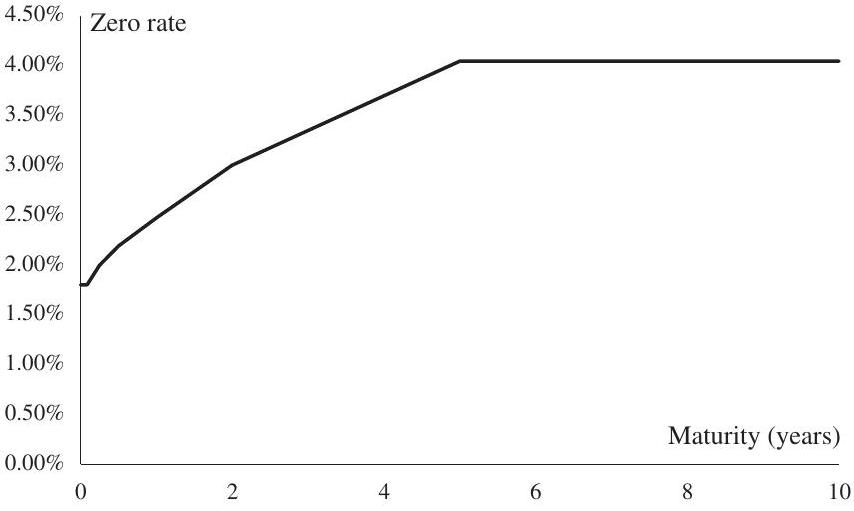
\includegraphics[width=\linewidth]{b71beec3-7c42-4186-a630-199cabe63c35-176_511_854_1798_457.jpg}
\caption{A zero curve gives the discounting input for each maturity. The shape
of the curve matters because fixed-income instruments usually contain cash
flows on many dates.}
\end{marginfigure}

\subsection{Bond Pricing}

A coupon bond is a package of dated cash flows. If the bond pays cash flows
$C_i$ at dates $t_i$, its no-arbitrage value is
\[
    B=\sum_i C_i P(0,t_i).
\]
Using continuously compounded zero rates,
\[
    B=\sum_i C_i e^{-R(0,t_i)t_i}.
\]

\begin{boxD}
\textbf{Key distinction.} A bond's yield is a single internal rate of return
that prices the entire bond. A zero curve is a term structure of rates that
prices each cash flow at its own maturity. Derivative valuation usually needs
the zero curve.
\end{boxD}

\subsection{Bond Yield}

The yield to maturity is the single discount rate $y$ that makes the present
value of the bond's promised cash flows equal to its market price:
\[
    B=\sum_i C_i e^{-y t_i}
\]
when $y$ is continuously compounded. The yield is useful as a summary statistic,
but it hides the term structure. Two bonds with the same yield can have very
different interest-rate sensitivities.

\section{Bootstrapping a Zero Curve}

\subsection{The Bootstrap Logic}

Bootstrapping uses traded instruments one maturity at a time. Short-maturity
cash instruments pin down early discount factors. Then longer coupon bonds,
FRAs, futures, or swaps pin down later discount factors after the earlier ones
are already known.

The logic is recursive:
\begin{enumerate}
    \item Start with the shortest maturity instrument.
    \item Use its price to infer the first discount factor.
    \item Move to the next maturity.
    \item Subtract the present value of earlier cash flows using already known
    discount factors.
    \item Solve for the new discount factor.
\end{enumerate}

\begin{exmp}[A simple bootstrap]
A six-month zero-coupon bond with face value 100 costs 98. Its discount factor
is
\[
    P(0,0.5)=0.98.
\]
The continuously compounded six-month zero rate is
\[
    R(0,0.5)=-\frac{1}{0.5}\ln(0.98)\approx 4.04\%.
\]

Now suppose a one-year bond costs 101 and pays 3 in six months and 103 in one
year. The one-year discount factor solves
\[
    101=3P(0,0.5)+103P(0,1).
\]
Using $P(0,0.5)=0.98$,
\[
    P(0,1)=\frac{101-3(0.98)}{103}\approx 0.9511.
\]
The one-year continuously compounded zero rate is
\[
    R(0,1)=-\ln(0.9511)\approx 5.01\%.
\]
\end{exmp}

\begin{boxF}
\textbf{Numerical discipline.} Bootstrapping is sensitive to conventions:
clean versus dirty prices, accrued interest, day count, coupon frequency,
settlement dates, holidays, and interpolation rules. The formula is simple; the
market implementation is detailed.
\end{boxF}

\section{Forward Rates}

\subsection{Forward Rates from Zero Rates}

A forward rate is a rate agreed today for borrowing or lending over a future
period. Under continuous compounding, the forward rate from $T_1$ to $T_2$ is
the rate $F(T_1,T_2)$ that makes investing to $T_2$ directly equivalent to
investing to $T_1$ and then rolling over at the forward rate:
\[
    e^{R(0,T_2)T_2}
    =
    e^{R(0,T_1)T_1}e^{F(T_1,T_2)(T_2-T_1)}.
\]
Therefore
\[
    F(T_1,T_2)
    =
    \frac{R(0,T_2)T_2-R(0,T_1)T_1}{T_2-T_1}.
\]

In discount-factor form,
\[
    e^{-F(T_1,T_2)(T_2-T_1)}
    =
    \frac{P(0,T_2)}{P(0,T_1)}.
\]

\begin{exmp}[Forward rate from two zero rates]
The one-year zero rate is 3\% and the two-year zero rate is 4\%, both with
continuous compounding. The one-year forward rate for the second year is
\[
    F(1,2)=\frac{0.04(2)-0.03(1)}{2-1}=0.05.
\]
The second-year forward rate is 5\%.
\end{exmp}

\subsection{Interpretation}

Forward rates are break-even rates implied by the current zero curve. They are
not generally unbiased forecasts of future spot rates. They include risk
premia, convexity effects, liquidity effects, and market segmentation. In
pricing, we use them because they are arbitrage-consistent with current market
prices.

\section{Forward Rate Agreements}

\subsection{FRA Mechanics}

A forward rate agreement (FRA) locks in an interest rate for a future borrowing
or lending period. The notional is not exchanged. At the reset date, the market
rate for the period is observed and one party compensates the other for the
difference between the market rate and the contract rate.

Let:
\begin{itemize}
    \item $\notional$ be the notional principal;
    \item $K$ be the FRA contract rate;
    \item $R$ be the market rate observed at the reset date;
    \item $\tau$ be the accrual fraction for the underlying loan period.
\end{itemize}

For the party that receives floating and pays fixed, the payoff paid at the
reset date is commonly written as
\[
    \frac{\notional \tau (R-K)}{1+R\tau}.
\]
The denominator discounts the payoff from the end of the underlying loan period
back to the reset date.

\begin{exmp}[FRA settlement]
A trader has an FRA to receive floating and pay fixed on notional EUR 20
million. The contract rate is 4.00\%, the realized reference rate is 4.60\%,
and the accrual period is three months, so $\tau=0.25$. The settlement at the
reset date is
\[
    \frac{20{,}000{,}000(0.25)(0.046-0.040)}
    {1+0.046(0.25)}
    \approx 29{,}659.
\]
The payoff is positive because the trader locked in paying 4.00\% and the
market rate moved to 4.60\%.
\end{exmp}

\section{Duration}

\subsection{Macaulay Duration}

Duration measures the weighted average timing of a bond's cash flows and the
first-order sensitivity of bond value to yield changes. With continuous
compounding, if a bond price is
\[
    B=\sum_i C_i e^{-y t_i},
\]
then Macaulay duration is
\[
    \Dur=\frac{\sum_i t_i C_i e^{-y t_i}}{B}.
\]

Differentiating the bond price with respect to $y$ gives
\[
    \frac{\Delta B}{B}\approx -\Dur \Delta y.
\]
Longer-duration bonds lose more value when yields rise and gain more value when
yields fall.

\begin{exmp}[Duration of a two-cash-flow bond]
A bond pays 5 in one year and 105 in two years. The continuously compounded
yield is 4\%. Its price is
\[
    B=5e^{-0.04}+105e^{-0.08}\approx 101.78.
\]
Its duration is
\[
    \Dur=
    \frac{1(5e^{-0.04})+2(105e^{-0.08})}{101.78}
    \approx 1.95.
\]
For a 20 basis point parallel yield increase, the duration approximation gives
\[
    \frac{\Delta B}{B}\approx -1.95(0.002)=-0.0039,
\]
or a price decline of about 0.39\%.
\end{exmp}

\subsection{Modified Duration}

When yields are quoted with periodic compounding, the price sensitivity is
usually stated using modified duration. If Macaulay duration is $D$ and the
yield is compounded $m$ times per year, then
\[
    D^*=\frac{D}{1+y/m}.
\]
The approximation becomes
\[
    \frac{\Delta B}{B}\approx -D^* \Delta y.
\]

\subsection{Portfolio Duration}

The duration of a portfolio is the value-weighted average of the durations of
its components:
\[
    D_P=\sum_j w_j D_j,
\]
where $w_j$ is the fraction of portfolio value invested in instrument $j$.
This lets a manager estimate interest-rate exposure at the portfolio level.

\section{Convexity}

\subsection{Why Duration Is Not Enough}

Duration is a linear approximation. Bond prices are curved functions of yields:
as yields fall, price gains accelerate; as yields rise, price losses are
smaller than a purely linear approximation would predict for sufficiently large
moves.

\begin{marginfigure}
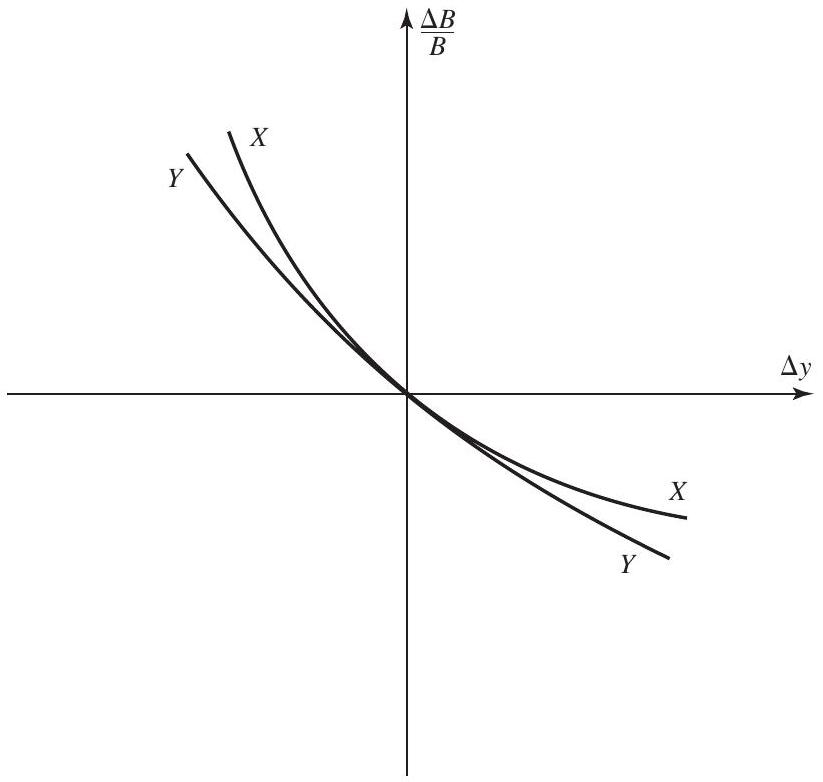
\includegraphics[width=\linewidth]{b71beec3-7c42-4186-a630-199cabe63c35-116_782_823_1490_455.jpg}
\caption{Duration is the tangent-line approximation. Convexity captures the
curvature of the bond price-yield relation.}
\end{marginfigure}

With continuous compounding, convexity is
\[
    \Conv=\frac{\sum_i t_i^2 C_i e^{-y t_i}}{B}.
\]
The duration-convexity approximation is
\[
    \frac{\Delta B}{B}
    \approx
    -\Dur\Delta y+\frac{1}{2}\Conv(\Delta y)^2.
\]

\begin{exmp}[Adding convexity]
Suppose a bond has duration 6.8 and convexity 55. If yields increase by 50
basis points, $\Delta y=0.005$. The duration-only approximation is
\[
    -6.8(0.005)=-3.40\%.
\]
The convexity correction is
\[
    \frac{1}{2}(55)(0.005)^2=0.0006875,
\]
or 0.06875\%. The duration-convexity approximation is therefore
\[
    -3.40\%+0.06875\%=-3.33125\%.
\]
\end{exmp}

\section{Term Structure Theories}

The zero curve contains market information, but its shape can be interpreted in
several ways.
\begin{description}
    \item[Expectations theory] Forward rates reflect expected future short
    rates.
    \item[Market segmentation] Different investors and borrowers concentrate
    on different maturities, so supply and demand by maturity affects yields.
    \item[Liquidity preference] Investors may require compensation for holding
    longer-maturity bonds, creating a term premium.
\end{description}

For derivative pricing, the most important point is not choosing one theory.
It is using a curve that is internally consistent with market prices and then
being clear about whether a forward rate is a pricing rate or a forecast.

\section{Interest Rate Futures}

\subsection{Day Count and Quotation Conventions}

Fixed-income markets are convention-heavy. Interest accruals depend on the day
count convention. Common examples include actual/actual, actual/360, and
30/360. The same quoted annual rate can imply different cash interest over a
calendar period if the day count differs.

\begin{boxF}
\textbf{Do not ignore conventions in implementation.} In classroom derivations
we often simplify by assuming exact year fractions. In market pricing, small
differences in day count, settlement, accrued interest, and holiday calendars
can change the quoted price and the hedge.
\end{boxF}

\subsection{Treasury Bill and Bond Quotes}

Treasury bills are discount instruments and are often quoted using bank discount
rates. Treasury bonds are coupon instruments and are usually quoted as clean
prices. The invoice amount paid by a buyer is the dirty price:
\[
    \text{dirty price}=\text{clean price}+\text{accrued interest}.
\]

The distinction matters for futures delivery and bond pricing because actual
cash paid at settlement includes accrued interest.

\section{Treasury Bond Futures}

\subsection{The Delivery Option}

Treasury bond futures allow the short futures position to choose from a basket
of deliverable bonds. Because different deliverable bonds have different
coupons and maturities, the exchange uses conversion factors to standardize
delivery.

\begin{defN}[Conversion factor]
The conversion factor adjusts the invoice price of a deliverable bond in a
Treasury bond futures contract. Ignoring accrued interest, the invoice price is
approximately
\[
    \text{futures quote}\times \CF.
\]
\end{defN}

The full invoice amount is
\[
    \text{invoice amount}
    =
    \text{futures settlement price}\times \CF
    +\text{accrued interest}.
\]

\subsection{Cheapest-to-Deliver}

The short chooses the bond that is cheapest to deliver. Ignoring accrued
interest and delivery timing details, the short compares
\[
    \text{cash bond price}-(\text{futures price})\times \CF.
\]
The bond with the lowest cost is the cheapest-to-deliver bond.

\begin{exmp}[Cheapest-to-deliver comparison]
The futures price is 112. Three deliverable bonds have clean prices and
conversion factors:
\[
\begin{array}{lcc}
\toprule
\text{Bond} & \text{Cash price} & \CF \\
\midrule
A & 118.20 & 1.0500 \\
B & 124.40 & 1.1030 \\
C & 110.10 & 0.9800 \\
\bottomrule
\end{array}
\]
Ignoring accrued interest, the delivery costs are
\[
\begin{aligned}
A &: 118.20-112(1.0500)=0.60,\\
B &: 124.40-112(1.1030)=0.864,\\
C &: 110.10-112(0.9800)=0.34.
\end{aligned}
\]
Bond C is cheapest to deliver.
\end{exmp}

\subsection{Futures Price from a Known CTD Bond}

If the cheapest-to-deliver bond is known and delivery options are ignored, the
futures price can be approximated from cost of carry:
\[
    F_0 \approx \frac{(B_0-I)e^{rT}}{\CF},
\]
where $B_0$ is the current dirty price of the CTD bond, $I$ is the present value
of coupons received before delivery, $r$ is the financing rate, $T$ is time to
delivery, and $\CF$ is the conversion factor.

\begin{boxD}
\textbf{Connection to Lecture 2.} Treasury bond futures use the same
cash-and-carry logic as forwards on investment assets. The added complications
are coupons, accrued interest, conversion factors, and delivery options.
\end{boxD}

\section{SOFR Futures}

\subsection{Reference Rate Futures}

Short-term interest-rate futures settle on reference rates. Older textbooks and
market histories discuss Eurodollar futures, which were linked to three-month
LIBOR. The post-LIBOR U.S. market uses SOFR futures, based on the secured
overnight financing rate.

A standard interest-rate futures quote is often written as
\[
    \text{futures quote}=100-\text{annualized rate}.
\]
Thus a quote of 95.25 corresponds to an implied rate of 4.75\%.

\begin{exmp}[SOFR futures quote]
A SOFR futures quote is 96.80. The implied annualized rate is
\[
    100-96.80=3.20\%.
\]
If the quote falls to 96.65, the implied rate rises to 3.35\%. A falling price
therefore corresponds to rising interest-rate expectations.
\end{exmp}

\subsection{Compounding and Convexity}

SOFR for a longer period is built from overnight rates compounded over the
period. The annualized compounded rate has the form
\[
    \left[\prod_{i=1}^n \left(1+r_i\frac{d_i}{360}\right)-1\right]
    \frac{360}{D},
\]
where $r_i$ is the annualized overnight rate for day $i$, $d_i$ is the number
of calendar days covered by that rate, and $D=\sum_i d_i$.

Futures rates and forward rates are not always identical because futures are
settled daily. Daily settlement creates a convexity effect when the futures
payoff is correlated with interest rates. For short maturities the adjustment
may be small; for longer maturities and volatile rates it can matter.

\section{Duration-Based Hedging with Futures}

\subsection{Hedging a Bond Portfolio}

A bond portfolio loses value when yields rise. A manager can hedge by shorting
interest-rate futures. If rates rise, the bond portfolio loses value but the
short futures position gains.

For a portfolio value $P$ with duration $D_P$, and a futures contract with price
$F$ and duration $D_F$ for the asset underlying the futures contract, the hedge
ratio is approximately
\[
    N^*=\frac{P D_P}{F D_F}.
\]
If the portfolio yield and the futures-implied yield do not move one-for-one,
include a yield beta:
\[
    N^*=\frac{P D_P}{F D_F}
    \frac{\Delta y_P}{\Delta y_F}.
\]

\begin{exmp}[Duration hedge]
A bond portfolio is worth EUR 40 million and has duration 5.5. The futures
contract price is EUR 120,000 and the duration of the deliverable bond exposure
is 7.2. Assuming parallel yield moves,
\[
    N^*=\frac{40{,}000{,}000(5.5)}
    {120{,}000(7.2)}
    \approx 254.6.
\]
The manager shorts about 255 futures contracts.
\end{exmp}

\subsection{Limits of Duration Hedges}

Duration hedging is approximate. It assumes small yield changes, stable
duration, parallel shifts, and a reliable relationship between the portfolio
yield and the futures yield. The hedge can fail when the yield curve twists,
credit spreads move, the cheapest-to-deliver bond changes, or convexity is
important.

\section{Interest Rate Swaps}

\subsection{Plain Vanilla Swap Mechanics}

A plain vanilla interest rate swap exchanges fixed interest payments for
floating interest payments on a notional principal. The notional is used to
calculate interest but is not exchanged.

In a fixed-for-floating swap:
\begin{itemize}
    \item one party pays a fixed rate $S$ on notional $\notional$;
    \item the other party pays a floating reference rate, such as compounded
    SOFR plus or minus a spread;
    \item payments are netted on each payment date.
\end{itemize}

\begin{marginfigure}
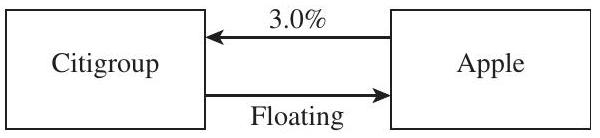
\includegraphics[width=\linewidth]{b71beec3-7c42-4186-a630-199cabe63c35-174_138_600_339_457.jpg}
\caption{A fixed-for-floating swap exchanges fixed-rate payments for floating
rate payments on the same notional.}
\end{marginfigure}

\begin{boxD}
\textbf{Economic use.} A borrower with floating-rate debt can enter a swap to
pay fixed and receive floating. The floating receipts offset the floating debt
payments, transforming the liability into a fixed-rate liability.
\end{boxD}

\subsection{Net Payments}

Suppose payments occur every $\tau$ years. If the fixed rate is $S$ and the
floating rate set for the period is $L$, the net payment from the fixed payer
to the floating payer is
\[
    \notional \tau (S-L).
\]
If $L>S$, the fixed payer receives the difference. If $S>L$, the fixed payer
pays the difference.

\section{The Swap Rate}

\subsection{Par Swap Rate}

At initiation, a standard swap is usually priced so that its value is zero. The
fixed rate that makes the value zero is the par swap rate.

Let payment dates be $T_1,\ldots,T_n$ with accrual fractions
$\alpha_1,\ldots,\alpha_n$. Let $P(0,T_i)$ be discount factors. For a standard
par swap with no exchange of principal, the fixed rate is
\[
    S=\frac{1-P(0,T_n)}
    {\sum_{i=1}^n \alpha_i P(0,T_i)}.
\]
The denominator is the fixed-leg annuity.

\begin{exmp}[Par swap rate]
A two-year swap pays annually. Discount factors are $P(0,1)=0.96$ and
$P(0,2)=0.915$. With $\alpha_1=\alpha_2=1$, the par fixed rate is
\[
    S=\frac{1-0.915}{0.96+0.915}
    =
    0.0453.
\]
The par swap rate is about 4.53\%.
\end{exmp}

\subsection{Relationship to the Zero Curve}

The swap rate is a weighted average of forward rates, where the weights are
discounted accrual factors. When the zero curve slopes upward, longer swap rates
usually exceed shorter rates. But the swap rate is not simply the zero rate for
the same maturity.

\section{Valuing Interest Rate Swaps}

\subsection{Bond Decomposition}

A fixed-for-floating interest rate swap can be valued as the difference between
a floating-rate bond and a fixed-rate bond.

For a party that receives floating and pays fixed,
\[
    V_{\text{swap}}=B_{\text{float}}-B_{\text{fixed}}.
\]
For a party that receives fixed and pays floating,
\[
    V_{\text{swap}}=B_{\text{fixed}}-B_{\text{float}}.
\]

The fixed-rate bond value is
\[
    B_{\text{fixed}}
    =
    \notional S\sum_{i=1}^n \alpha_i P(0,T_i)
    +\notional P(0,T_n).
\]
The floating-rate bond value is close to par immediately after a reset date.
Between reset dates, it equals the present value of the next known floating
payment plus principal.

\begin{exmp}[Swap value after rates change]
A EUR 10 million swap has one and two years remaining, annual payments, and
fixed rate 4.00\%. The current discount factors are $P(0,1)=0.955$ and
$P(0,2)=0.900$. For the party receiving fixed and paying floating, the fixed
bond value is
\[
\begin{aligned}
    B_{\text{fixed}}
    &=
    10{,}000{,}000(0.04)(0.955+0.900)\\
    &\quad +10{,}000{,}000(0.900)\\
    &=
    9{,}742{,}000.
\end{aligned}
\]
If the swap is just after a reset date, approximate
$B_{\text{float}}=10{,}000{,}000$. Then
\[
    V_{\text{receive fixed}}
    =
    9{,}742{,}000-10{,}000{,}000
    =
    -258{,}000.
\]
The receive-fixed position is negative because current rates have moved above
the old fixed rate.
\end{exmp}

\subsection{FRA Decomposition}

The same swap can be viewed as a portfolio of forward rate agreements. For a
receive-floating, pay-fixed swap, the value is approximately
\[
    V
    =
    \notional\sum_i \alpha_i (F_i-S)P(0,T_i),
\]
where $F_i$ is the forward rate for payment period $i$. This representation
makes clear that a swap locks in a sequence of future short-rate exchanges.

\section{Using Swaps to Transform Assets and Liabilities}

\subsection{Transforming a Liability}

Suppose a firm has floating-rate debt and wants fixed-rate debt. It can enter a
swap where it pays fixed and receives floating. The floating leg received on the
swap offsets the floating payments on the debt. The firm is left paying the
fixed swap rate plus any borrowing spread on its debt.

If the firm instead has fixed-rate debt and wants floating-rate exposure, it can
enter the opposite swap: receive fixed and pay floating.

\subsection{Transforming an Asset}

A bank that owns a fixed-rate loan can use a swap to receive floating and pay
fixed, thereby transforming a fixed-rate asset into a floating-rate asset. This
can help manage net interest income when liabilities reprice more quickly than
assets.

\begin{boxF}
\textbf{Risk-management point.} A swap changes interest-rate exposure, but it
does not eliminate all risk. Basis risk, credit risk, collateral liquidity,
model risk, and operational risk remain.
\end{boxF}

\section{Currency Swaps}

\subsection{Fixed-for-Fixed Currency Swaps}

In a currency swap, the parties exchange cash flows in different currencies.
Unlike a plain vanilla interest rate swap, the principals are usually exchanged
at the start and re-exchanged at maturity.

For example, one party might pay fixed dollars and receive fixed euros. The
currency swap value is the domestic value of one bond minus the domestic value
of the other bond. If $S_0$ is the domestic price of one unit of foreign
currency, then a receive-foreign, pay-domestic position has value
\[
    V=S_0 B_{\text{foreign}}-B_{\text{domestic}}.
\]

\subsection{Uses}

Currency swaps can transform borrowing from one currency into another, exploit
market access differences, and manage long-term foreign-currency cash-flow
exposure. They introduce exchange-rate exposure and cross-currency funding
spreads, so valuation requires both interest-rate curves and the spot exchange
rate.

\section{Credit Risk and Other Swaps}

\subsection{Credit Risk in Swaps}

A swap's credit exposure changes through time. At initiation, a standard swap
has value near zero, but later rate movements can make it positive to one party
and negative to the other. The party for whom the swap has positive value is
exposed to counterparty default.

Collateral agreements, central clearing, netting, and margin reduce this risk,
but they do not make it disappear. This is why modern derivative valuation often
distinguishes between the trade's promised cash flows and adjustments for
funding, collateral, capital, and counterparty credit risk.

\subsection{Other Swap Structures}

The same swap logic extends beyond standard interest rate swaps:
\begin{itemize}
    \item basis swaps exchange one floating rate for another;
    \item overnight indexed swaps exchange fixed payments for compounded
    overnight floating payments;
    \item equity swaps exchange equity-index returns for fixed or floating
    interest;
    \item commodity swaps exchange a fixed commodity price for a floating spot
    or index price;
    \item volatility swaps and variance swaps exchange payments linked to
    realized volatility or variance.
\end{itemize}

The valuation details differ, but the common structure is the same: identify
the future cash flows, choose the relevant state variables and discount curve,
and value the contract by no-arbitrage or a pricing model.

\section{Worked Problems}

\begin{exmp}[Discount factor from zero rate]
The continuously compounded two-year zero rate is 3.75\%. The discount factor
is
\[
    P(0,2)=e^{-0.0375(2)}=e^{-0.075}\approx 0.9277.
\]
Receiving EUR 1 million in two years is worth approximately
\[
    1{,}000{,}000(0.9277)=927{,}700.
\]
\end{exmp}

\begin{exmp}[Bond price from zero curve]
A bond pays 4 in one year and 104 in two years. The one-year zero rate is
3\% and the two-year zero rate is 3.8\%, both continuously compounded. The
price is
\[
    B=4e^{-0.03(1)}+104e^{-0.038(2)}
    \approx 3.88+96.38=100.26.
\]
\end{exmp}

\begin{exmp}[Forward rate from discount factors]
Suppose $P(0,1)=0.9704$ and $P(0,1.5)=0.9418$. The continuously compounded
forward rate from year 1 to year 1.5 solves
\[
    e^{-F(0.5)}=\frac{0.9418}{0.9704}.
\]
Thus
\[
    F=-\frac{1}{0.5}\ln\left(\frac{0.9418}{0.9704}\right)
    \approx 6.0\%.
\]
\end{exmp}

\begin{exmp}[Treasury bond futures approximation]
The dirty price of the CTD bond is 128.50. Coupons with present value 2.10 will
be received before delivery. The financing rate is 4\%, time to delivery is
0.5 years, and the conversion factor is 1.18. The approximate futures price is
\[
    F_0=\frac{(128.50-2.10)e^{0.04(0.5)}}{1.18}
    =
    \frac{126.40e^{0.02}}{1.18}
    \approx 109.31.
\]
\end{exmp}

\begin{exmp}[Swap rate from discount factors]
A three-year swap pays annually. Discount factors are
\[
    P(0,1)=0.970,\quad P(0,2)=0.930,\quad P(0,3)=0.885.
\]
The par swap rate is
\[
    S=\frac{1-0.885}{0.970+0.930+0.885}
    =
    \frac{0.115}{2.785}
    \approx 4.13\%.
\]
\end{exmp}

\section{Checklist for Students}

After this lecture you should be able to:
\begin{itemize}
    \item explain why derivative pricing uses discount curves rather than one
    universal interest rate;
    \item convert rates across compounding frequencies;
    \item compute continuously compounded discount factors;
    \item define zero rates, par yields, and forward rates;
    \item price a coupon bond from a zero curve;
    \item bootstrap a simple zero curve from bond prices;
    \item calculate forward rates from zero rates or discount factors;
    \item explain the settlement logic of a forward rate agreement;
    \item compute duration and use it for first-order interest-rate risk;
    \item add convexity to improve the price-change approximation;
    \item distinguish clean price, dirty price, and accrued interest;
    \item explain conversion factors and cheapest-to-deliver logic in Treasury
    bond futures;
    \item interpret SOFR futures quotes;
    \item construct a duration-based futures hedge for a bond portfolio;
    \item describe fixed-for-floating swap cash flows;
    \item derive the par swap rate from discount factors;
    \item value a swap as the difference between a fixed-rate bond and a
    floating-rate bond;
    \item explain how swaps transform assets and liabilities;
    \item identify the main risks that remain after entering an interest-rate
    swap.
\end{itemize}

\section{Practice Questions}

\begin{enumerate}
    \item Convert a rate of 8\% compounded quarterly into an equivalent
    continuously compounded rate.
    \item Convert a continuously compounded rate of 5\% into an equivalent
    semiannually compounded rate.
    \item A three-year zero rate is 4.2\% with continuous compounding. Compute
    the three-year discount factor.
    \item A bond pays 6 in one year and 106 in two years. The one-year and
    two-year zero rates are 3\% and 4\%. Compute the bond price.
    \item A six-month zero-coupon bond costs 97.80 per 100 face value. Compute
    the six-month continuously compounded zero rate.
    \item A one-year coupon bond costs 101.20 and pays 4 in six months and 104
    in one year. Use the discount factor from the previous question to bootstrap
    the one-year discount factor.
    \item The one-year zero rate is 3.5\% and the two-year zero rate is 4.1\%,
    both continuously compounded. Compute the one-year forward rate for year 2.
    \item A trader receives floating and pays fixed in an FRA. The notional is
    50 million, the contract rate is 3.7\%, the realized rate is 4.1\%, and the
    accrual fraction is 0.25. Compute the settlement at the reset date.
    \item A bond pays 3 in one year and 103 in two years. Its continuously
    compounded yield is 4.5\%. Compute its price and duration.
    \item A bond has duration 8 and convexity 80. Approximate the percentage
    price change when yields rise by 25 basis points.
    \item Explain why a high-convexity bond is more valuable than a low-convexity
    bond with the same price and duration, holding other risks fixed.
    \item A Treasury bond futures price is 118. One deliverable bond has price
    126 and conversion factor 1.060. Another has price 121 and conversion
    factor 1.020. Which is cheaper to deliver, ignoring accrued interest?
    \item The dirty price of the CTD bond is 115. Coupons with present value 1.5
    are paid before delivery, the financing rate is 3\%, delivery is in four
    months, and the conversion factor is 0.92. Approximate the futures price.
    \item A SOFR futures quote falls from 95.40 to 95.10. What happens to the
    implied rate?
    \item A bond portfolio is worth USD 25 million and has duration 6. A futures
    contract has price USD 110,000 and duration 7.5. Compute the approximate
    number of contracts for a duration hedge.
    \item Draw the cash flows for a party that pays fixed and receives floating
    in an interest rate swap.
    \item Annual discount factors for years 1, 2, and 3 are 0.965, 0.925, and
    0.880. Compute the three-year annual-pay par swap rate.
    \item A receive-fixed swap has fixed rate 5\%, notional 20 million, and two
    annual payments remaining. Current discount factors are 0.96 and 0.91. If
    the floating-rate bond value is approximately par, compute the swap value.
    \item Explain why a swap can have zero value at initiation but large credit
    exposure later.
    \item Give one example each of an interest rate swap, a basis swap, a
    currency swap, and a commodity swap.
\end{enumerate}

\end{document}
